\documentclass[11pt]{article}

\usepackage{amsmath}
\usepackage{amsfonts} 
\usepackage{amsthm}
\usepackage{blkarray}
\usepackage{caption}
\usepackage{enumitem} 
\usepackage{mathtools}
\usepackage{tikz}
\usepackage[top=2cm,bottom=2cm,left=2cm,right=2cm,marginparwidth=1.75cm]{geometry}
\setlength{\parindent}{0cm}

\newcommand{\R}{\mathbb{R}}
\newcommand\simpleGraph[1]{
  \begin{tikzpicture}[every node/.style={circle,draw}]
    \node (a) at (0,1) {};
    \node (b) at (1,1) {};
    \node (c) at (1,0) {};
    \node (d) at (0,0) {};

    \foreach \from/\to in {#1}
      \draw (\from) -- (\to);
  \end{tikzpicture}\hfil
}
\newcommand\itm[1]{\item[\textbf{#1}]}
\newcommand{\incid}{{-}\!{\bullet}\!{-}}
\newcommand{\n}{\vspace{0.5cm}}

\newtheorem{theorem}{Theorem}

\title{\vspace{-1.0cm}MATH 5707 Homework 1}
\author{Fletcher Gornick}
\date{January 18, 2022}

\begin{document}
\maketitle
\begin{itemize}
  \itm{1.2.4} Show that there are eleven nonisomorphic simple graphs on four vertices.

    \simpleGraph{}
    \simpleGraph{a/b}
    \simpleGraph{a/b,a/d}
    \simpleGraph{a/d,b/c}
    \simpleGraph{a/b,a/c,a/d}
    \simpleGraph{a/d,a/b,b/c}

    \simpleGraph{a/b,a/d,b/d}
    \simpleGraph{a/b,b/c,c/d,d/a}
    \simpleGraph{a/b,b/d,c/d,d/a}
    \simpleGraph{a/b,b/c,c/d,d/a,a/c}
    \simpleGraph{a/b,b/c,c/d,d/a,a/c,b/d}



  \itm{1.2.10} The \textit{\(k\)-cube} is the graph whose vertices are the ordered \(k\)-tuples of 0's and 1's, two vertices being joined if and only if they differ in exactly one coordinate.  Show that the \(k\)-cube has \(2^k\) vertices, \(k 2^{k-1}\) edges and is bipartite.

    \begin{proof}
      any \(k\)-length binary string has \(2^k\) possible combinations (2 choices \(k\) times), so there are clearly \(2^k\) vertices.

      For each vertex represented by a binary string, we can change one bit anywhere in the string producing a new vertex in our set differing in exactly one coordinate, and since it's a \(k\)-length binary string, we know that there are \(k\) different strings of hamming distance 1 from our original.  This tells us that every vertex has degree \(k\) (\(k\)-cube is also \(k\)-regular).

      From theorem 1.1, assuming our graph \(G = (V,E)\), \(|V| = \nu = 2^k\) and \(|E| = \varepsilon\), we know that \(\displaystyle\sum_{v \in V} d_G(v) = 2\varepsilon\), so we can plug in \(d_G(v) = k\) for each \(v \in G\), because \(G\) is \(k\)-regular, giving us \(2^k \cdot k = \displaystyle\sum_{v \in V} k = \displaystyle\sum_{v \in V} d_G(v) = 2\varepsilon\).  This tells us that the \(k\)-cube has \(k \cdot 2^{k-1}\) edges.

      Finally, to show the \(k\)-cube is bipartite, we can split the vertices into groups \(V_1\) and \(V_2\).  \(V_1\) will consist of all the vertices with an even \textit{parity} (number of 1's in it's tuple representation), and \(V_2\) will consist of vertices with an odd parity.  Clearly, vertices can only be adjacent to eachother if they have differing parities (otherwise they would be the same vertex, or their hamming distance would be \(\geq 2\)), so the only edges that can exist (in a \(k\)-cube) go between \(V_1\) and \(V_2\).  Thus the \(k\)-cube must be bipartite.
    \end{proof}



  \itm{1.2.11} \begin{enumerate}[label=(\alph*)]
      \item The \textit{complement} \(G^c\) of a simple graph \(G\) is the simple graph with vertex set \(V\), two vertices being adjacent in \(G^c\) if and only if they are not adjacent in \(G\). Describe the graphs \(K^c_n\) and \(K^c_{m,n}\). \n

        The graph of \(K_n^c\) is just the empty graph with \(n\) vertices.  Since every vertex is adjacent to another in \(K_n\), none are in it's complement. \n

        For the graph of \(K_{m,n}^c\), it will consist of two edge-distinct complete graphs \(K_m\) and \(K_n\).  
        \begin{proof}
          First split \(K_{m,n}\) into two subsets \(V_m\) and \(V_n\).  Since \(K_{m,n}\) is a complete bipartite graph, every node in \(V_m\) is adjacent to every node in \(V_n\), therefore none are in it's complement.  Finally, since no vertex in \(V_m\) is adjacent to another in \(V_m\), every vertex is adjacent to every other vertex in it's complement (and similarly for \(V_n\)).  Thus, we get two edge-distinct complete graphs for the complement of a complete bipartite graph.
        \end{proof}

      \item A simple graph \(G\) is \textit{self-complementary} if \(G \cong G^c\). Show that if \(G\) is self-complementary, then \(\nu \equiv 0,1 \pmod 4\)
        \begin{proof}
          A complete graph has \(\displaystyle\binom\nu2\) edges (number of 2-element subsets of \(\{1,2,\hdots,\nu\}\)).  Assuming \(G\) is a spanning subgraph of \(K_\nu\), Then it must be true that \(|E(G)| + |E(G^c)| = |E(K_\nu)| = \displaystyle\binom\nu2 = \frac{\nu(\nu-1)}{2}\).

          For a graph to be self-complementary, it must also be true that \(|E(G)| = |E(G^c)|\) (otherwise \(\varphi \colon E(G) \to E(G^c)\) cannot be bijective), so we can rewrite the above equation to get that \(4|E(G)| = \nu(\nu-1)\)

          Now if \(\nu \equiv 2 \pmod 4\), then \(\nu = 4k+2\) for some \(k \in \mathbb{N}\). So \(\nu(\nu-1) = 4(4k^2 + 3k) + 3\) which is not a multiple of 4.

          For \(\nu \equiv 3 \pmod 4\), \(\nu = 4k+3\) for some \(k \in \mathbb{N}\), meaning \(\nu(\nu-1) = 4(4k^2 + 5k + 1) + 2\).  Again, not a multiple of 4, so unless there's not a whole number of edges, it must be the case that \(\nu \equiv 0,1 \pmod 4\) for a self-complementary graph.
        \end{proof}
    \end{enumerate}



  \itm{1.4.4} Find a bipartite graph that is not isomorphic to a subgraph of any \(k\)-cube.

    \begin{center}
      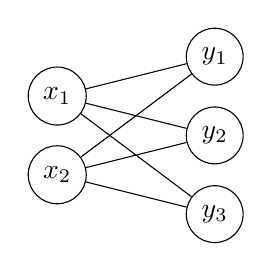
\begin{tikzpicture}[every node/.style={circle,draw}]
        \node (y1) at (0,1.5) {\(x_1\)};
        \node (y2) at (0,0.5) {\(x_2\)};
        \node (x1) at (2,2) {\(y_1\)};
        \node (x2) at (2,1) {\(y_2\)};
        \node (x3) at (2,0) {\(y_3\)};

        \draw (x1) -- (y1) -- (x2) -- (y2) -- (x3) -- (y1);
        \draw (x1) -- (y2);
      \end{tikzpicture}
    \end{center}

    take this bipartite graph for example.  We can denote the vertices of a \(k\)-cube with \(k\)-length binary strings, and edges only connecting vertices with a hamming distance of 1.  We show that 2 distinct vertices cannot be adjacent to the same 3 vertices in any \(k\)-cube.
      \begin{proof}
        Let \(d \colon V^2 \to \mathbb{N} \cup \{0\}\) denote the hamming distance between any two vertices.  if \(d(x_1,x_2) = 0\) then \(x_1 = x_2\), but we wish to deal only with distinct vertices, so assume \(d(x_1,x_2) \geq 1\). \n

        \(d(x_1, x_2) = 1\): In this case we have that \(x_1\) and \(x_2\) are adjacent to eachother.  WLOG, flip any bit in \(x_1\) (excluding the bit flip that leads to \(x_2\)), and call it \(x_3\).  We know \(x_1\) is adjacent to \(x_3\), but \(d(x_2,x_3) = 2\), meaning \(x_1\) and \(x_2\) share no extra adjacent node, so they certainly can't share 3. \n

        \(d(x_1,x_2) = 2\): In this case, \(x_1\) and \(x_2\) differ by two bits.  If we flip either of the bits they differ in (but not both), we get a new vertex adjacent to both \(x_1\) and \(x_2\).  This gives us 2 vertices adjacent to both \(x_1\) and \(x_2\).  But again, WLOG, if we flip any bit other than those two in \(x_1\) and call it \(x_3\), we get that \(d(x_2,x_3) = 3\), so there can exist no more than two nodes adjacent to both \(x_1\) and \(x_2\) in this case. \n

        \(d(x_1,x_2) \geq 3\): Finally, in this case it doesn't matter what bit we shift.  Shifing one bit in \(x_1\) and calling it \(x_3\) results in \(d(x_2,x_3) \geq 2\), so \(x_2\) can never be adjacent to the same node as \(x_1\) with hamming distance \(\geq 3\). \n

        In conclusion, for any \(k\)-cube, two vertices cannot be adjacent to the same 3 vertices, meaning that the above bipartite graph cannot be a subgraph of any \(k\)-cube.
      \end{proof}



  \itm{1.5.5} If \(G\) has vertices \(v_1, v_2, \hdots, v_v\), the sequence \((d(v_1), d(v_2), \hdots, d(v_v))\) is called a \textit{degree sequence} of \(G\).  Show that a sequence (\(d_1, d_2, \hdots, d_n\)) of non-negative integers is a degree sequence of some graph if and only if \(\displaystyle \sum_{i=1}^n d_i\) is even.
    \begin{proof}
      By theorem 1.1, \(\displaystyle\sum_{v \in V} d(v) = 2\varepsilon\), so it's clear that if \((d(v_1), d(v_2), \hdots, d(v_v))\) is a sequence of some graph, it must have an even sum. \n

      Conversely, to show that every degree sequence with even sum can be represented by a graph, we proceed inductively.

      First, suppose we have a degree sequence consisting of just one entry, \(d_1\).  Clearly \(d_1\) must be even, so we can construct a graph consising of \(\displaystyle\frac{d_1}{2}\) loops.

      For any 2-length degree sequence \((d_1,d_2)\), if \(d_1\) and \(d_2\) are both even then we can create a graph where one vertex has \(\displaystyle\frac{d_1}{2}\) loops and the other has \(\displaystyle\frac{d_2}{2}\) loops.  If \(d_1\) and \(d_2\) are odd then we can create a graph where one vertex has \(\displaystyle\frac{d_1-1}{2}\) loops, the other has \(\displaystyle\frac{d_2-1}{2}\) loops, and one link connects the two vertices.

      Now assume every nonnegative degree sequence \((d_1,d_2,\hdots,d_k)\) with \(\displaystyle\sum_{i=1}^{k}d_i\) even is graphic, as well as any smaller degree sequence (strong induction).  We show that every \((k+1)\)-length degree sequence with even sum must also be graphic.

      If \(d_{k+1}\) is even, \(\displaystyle\sum_{i=1}^{k}d_i\) must also be even (otherwise the new sum is odd), so we can just take the graph represented by \((d_1,d_2,\hdots,d_k)\) and add a single node with \(\displaystyle\frac{d_{k+1}}{2}\) loops and we're done.

      Otherwise, if \(d_{k+1}\) is odd, \(\displaystyle\sum_{i=1}^{k}d_i\) must also be odd.  This tells us that at least one of the degrees in \((d_1,d_2,\hdots,d_k)\) is odd as well, call it \(d_j\) (\(1 \leq j \leq k\)).  Now construct a new \((k-1)\)-length sequence consisting of all degrees in our \((k+1)\)-length sequence excluding \(d_j\) and \(d_{k+1}\).  Our new \((k-1)\)-length sequence now has an even sum, so it's graphic by our inductive hypothesis.  We can also create sequence \((d_j, d_{k+1})\) with even sum, so it must be graphic as well (length 2).  Finally, we can just take the union of the two distinct graphs represented by our two sequences to get a new graph represented by degree sequence \((d_1,d_2,\hdots,d_{k+1})\). \n

      Therefore, by the principle of strong mathematical induction, every \(k\)-length degree sequence with even sum is graphic, so the statement above must hold.
    \end{proof}


  \itm{1.5.7(a)} Let \(\textbf{d} = (d_1, d_2, \hdots, d_n)\) be a nonincreasing sequence of non-negative integers, and denote the sequence \((d_2-1, d_3-1, \hdots, d_{d_1+1}-1, d_{d_1+2}-1, \hdots, d_n)\) by \(\textbf{d'}\).  Show that \(\textbf{d}\) is graphic if and only if \(\textbf{d'}\) is graphic.

  doesn't the degree sequence \(\textbf{d}\) need to consist of strictly positive integers?  Otherwise I could just write a degree sequence consisting of all zeros which is obviously graphic (just an empty graph), but then \(\textbf{d'}\) would have negative degrees which can't be graphic. so \(\textbf{d}\) being graphic does not imply \(\textbf{d'}\) graphic.



  \itm{1.5.10} The \textit{edge graph} of a graph \(G\) is the graph with vertex set \(E(G)\) in which two vertices are joined if and only if they are adjacent edges in \(G\).  Show that, if \(G\) is simple
    \begin{enumerate}[label=(\alph*)]
      \item the edge graph of \(G\)  has \(\varepsilon(G)\) vertices and \(\displaystyle\sum_{v \in V(G)} \binom{d_G(v)}{2}\) edges;
        \begin{proof}
          obviously the edge graph of \(G\) (call it \(G'\)) will have \(\varepsilon(G)\) vertices, because our new vertex set is just the edge set of \(G\).

          As for the number of edges, let's look at each vertex in the original graph separately.  First, note that each vertex \(v \in V(G)\) is incident to \(d_G(v)\) edges (no loops because \(G\) is simple).  All the edges incident to \(v\) must be adjacent to eachother (by definition).

          Let \(S = \{e \in E(G) \mid e \incid v\}\) be the set of edges incident to \(v\).  The induced subgraph \(G'[S]\) is complete (edges adjacent in \(G\) \(\implies\) vertices adjacent in \(G'\)), so there are \(\displaystyle\binom{d_G(v)}{2}\) edges in \(G'[S]\).

        Finally, since \(G\) is simple, there does not exist any double links, so if 2 edges are adjacent to eachother through one vertex, they cannot be adjacent through another.  This tells us that each of the induced subgraphs of \(G'\) are edge-distinct, meaning 
        \[|E(G')| = \sum_{v \in V} G'[\{e \in E(G) \mid e \incid v\}] = \sum_{v \in V(G)} \binom{d_G(v)}{2}.\]
        \end{proof}
        
      \item the edge graph of \(K_5\) is isomorphic to the complement of the graph featured in exercise 1.2.6.
        \begin{figure}[!ht]
          \begin{minipage}{0.45\textwidth}
            \centering
            \resizebox{!}{4cm}{
              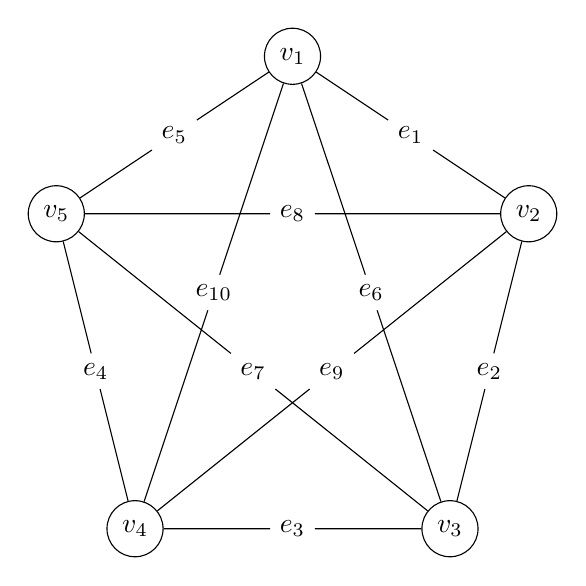
\begin{tikzpicture}
                \node[circle,draw] (v1) at (3,6) {\(v_1\)};
                \node[circle,draw] (v2) at (6,4) {\(v_2\)};
                \node[circle,draw] (v3) at (5,0) {\(v_3\)};
                \node[circle,draw] (v4) at (1,0) {\(v_4\)};
                \node[circle,draw] (v5) at (0,4) {\(v_5\)};

                \node (e1) at (4.5,5) {\(e_1\)};
                \node (e2) at (5.5,2) {\(e_2\)};
                \node (e3) at (3,0) {\(e_3\)};
                \node (e4) at (0.5,2) {\(e_4\)};
                \node (e5) at (1.5,5) {\(e_5\)};

                \node (e6) at (4,3) {\(e_6\)};
                \node (e7) at (2.5,2) {\(e_7\)};
                \node (e8) at (3,4) {\(e_8\)};
                \node (e9) at (3.5,2) {\(e_9\)};
                \node (e10) at (2,3) {\(e_{10}\)};

                \draw (v1) -- (e1) -- (v2) -- (e2) -- (v3) -- (e3) -- (v4) -- (e4) -- (v5) -- (e5) -- (v1);
                \draw (v1) -- (e6) -- (v3) -- (e7) -- (v5) -- (e8) -- (v2) -- (e9) -- (v4) -- (e10) -- (v1);
              \end{tikzpicture}
            }
            \captionsetup{labelformat=empty}
            \caption{\(K_5\) graph}
          \end{minipage}
          \(\Longrightarrow\)
          \begin{minipage}{0.45\textwidth}
            \centering
            \resizebox{!}{4cm}{
              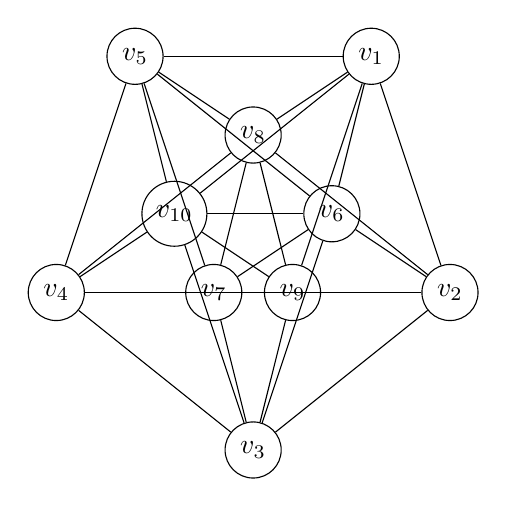
\begin{tikzpicture}
                \node[circle,draw] (v1) at (4.5,5) {\(v_1\)};
                \node[circle,draw] (v2) at (5.5,2) {\(v_2\)};
                \node[circle,draw] (v3) at (3,0) {\(v_3\)};
                \node[circle,draw] (v4) at (0.5,2) {\(v_4\)};
                \node[circle,draw] (v5) at (1.5,5) {\(v_5\)};
                \node[circle,draw] (v6) at (4,3) {\(v_6\)};
                \node[circle,draw] (v7) at (2.5,2) {\(v_7\)};
                \node[circle,draw] (v8) at (3,4) {\(v_8\)};
                \node[circle,draw] (v9) at (3.5,2) {\(v_9\)};
                \node[circle,draw] (v10) at (2,3) {\(v_{10}\)};

                \foreach \from/\to in {v9/v10,v8/v9,v7/v8,v6/v10,v6/v7,v5/v10,v5/v8,v5/v7,v5/v6,v4/v10,v4/v9,v4/v8,v4/v7,v4/v5,v3/v10,v3/v9,v3/v7,v3/v6,v3/v4,v2/v9,v2/v8,v2/v7,v2/v6,v2/v3,v1/v10,v1/v9,v1/v8,v1/v6,v1/v5,v1/v2}
                  \draw (\from) -- (\to);
              \end{tikzpicture}
            }
            \captionsetup{labelformat=empty}
            \caption{edge graph of \(K_5\)}
          \end{minipage}
          \vspace{1cm}

          \begin{minipage}{0.45\textwidth}
            \centering
            \resizebox{!}{2.5cm}{
              \begin{blockarray}{ccccccccccc}
                & \(e_1\) & \(e_2\) & \(e_3\) & \(e_4\) & \(e_5\) & \(e_6\) & \(e_7\) & \(e_8\) & \(e_9\) & \(e_{10}\) \\
                \begin{block}{c(cccccccccc)}
                  \(e_1\) & * & 1 & 0 & 0 & 1 & 1 & 0 & 1 & 1 & 1 \\
                  \(e_2\) & * & * & 1 & 0 & 0 & 1 & 1 & 1 & 1 & 0 \\
                  \(e_3\) & * & * & * & 1 & 0 & 1 & 1 & 0 & 1 & 1 \\
                  \(e_4\) & * & * & * & * & 1 & 0 & 1 & 1 & 1 & 1 \\
                  \(e_5\) & * & * & * & * & * & 1 & 1 & 1 & 0 & 1 \\
                  \(e_6\) & * & * & * & * & * & * & 1 & 0 & 0 & 1 \\
                  \(e_7\) & * & * & * & * & * & * & * & 1 & 0 & 0 \\
                  \(e_8\) & * & * & * & * & * & * & * & * & 1 & 0 \\
                  \(e_9\) & * & * & * & * & * & * & * & * & * & 1 \\
                  \(e_{10}\) & * & * & * & * & * & * & * & * & * & * \\
                \end{block}
              \end{blockarray}
            }
            \captionsetup{labelformat=empty}
            \caption{edge graph adjacency matrix}
          \end{minipage}
          \(\Longrightarrow\)
          \begin{minipage}{0.45\textwidth}
            \centering
            \resizebox{!}{2.5cm}{
              \begin{blockarray}{ccccccccccc}
                & \(e_1\) & \(e_2\) & \(e_3\) & \(e_4\) & \(e_5\) & \(e_6\) & \(e_7\) & \(e_8\) & \(e_9\) & \(e_{10}\) \\
                \begin{block}{c(cccccccccc)}
                  \(e_1\) & * & 0 & 1 & 1 & 0 & 0 & 1 & 0 & 0 & 0 \\
                  \(e_2\) & * & * & 0 & 1 & 1 & 0 & 0 & 0 & 0 & 1 \\
                  \(e_3\) & * & * & * & 0 & 1 & 0 & 0 & 1 & 0 & 0 \\
                  \(e_4\) & * & * & * & * & 0 & 1 & 0 & 0 & 0 & 0 \\
                  \(e_5\) & * & * & * & * & * & 0 & 0 & 0 & 1 & 0 \\
                  \(e_6\) & * & * & * & * & * & * & 0 & 1 & 1 & 0 \\
                  \(e_7\) & * & * & * & * & * & * & * & 0 & 1 & 1 \\
                  \(e_8\) & * & * & * & * & * & * & * & * & 0 & 1 \\
                  \(e_9\) & * & * & * & * & * & * & * & * & * & 0 \\
                  \(e_{10}\) & * & * & * & * & * & * & * & * & * & * \\
                \end{block}
              \end{blockarray}
            }
            \captionsetup{labelformat=empty}
            \caption{complement adjacency matrix}
          \end{minipage}
          \vspace{1cm}

          \begin{minipage}{\textwidth}
            \centering
            \resizebox{!}{4cm}{
              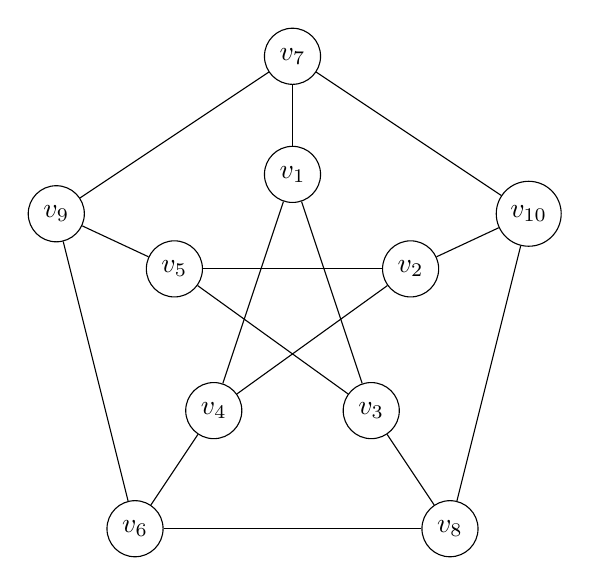
\begin{tikzpicture}
                \node[circle,draw] (v1) at (3,4.5) {\(v_1\)};
                \node[circle,draw] (v2) at (4.5,3.3) {\(v_2\)};
                \node[circle,draw] (v3) at (4,1.5) {\(v_3\)};
                \node[circle,draw] (v4) at (2,1.5) {\(v_4\)};
                \node[circle,draw] (v5) at (1.5,3.3) {\(v_5\)};
                \node[circle,draw] (v6) at (1,0) {\(v_6\)};
                \node[circle,draw] (v7) at (3,6) {\(v_7\)};
                \node[circle,draw] (v8) at (5,0) {\(v_8\)};
                \node[circle,draw] (v9) at (0,4) {\(v_9\)};
                \node[circle,draw] (v10) at (6,4) {\(v_{10}\)};

                \foreach \from/\to in {1/3,1/4,1/7,2/4,2/5,2/10,3/5,3/8,4/6,5/9,6/8,6/9,7/9,7/10,8/10}
                  \draw (v\from) -- (v\to);
              \end{tikzpicture}
            }
            \captionsetup{labelformat=empty}
            \caption{resulting graph (matching the one from 1.2.6)}
          \end{minipage}
        \end{figure}
    \end{enumerate}
    \newpage



  \itm{1.6.7} Show that if \(G\) is disconnected, then \(G^c\) is connected.



  \itm{1.6.10} Show that any two longest paths in a connected graph have a vertex in common.



  \itm{1.7.2} Show that if \(\delta \geq 2\), then \(G\) contains a cycle.



  \itm{4.1.1} Which of the following figures can be drawn without lifting one's pen from the paper or covering a line more than once?

    \resizebox{0.25\textwidth}{4cm}{
      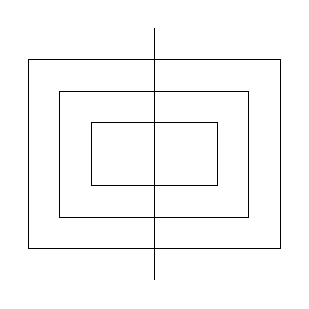
\begin{tikzpicture}[scale=0.4]
        \draw (4,0) -- (4,8);
        \draw (0,1) rectangle (8,7);
        \draw (1,2) rectangle (7,6);
        \draw (2,3) rectangle (6,5);
      \end{tikzpicture}
    }\hfil
    \resizebox{0.25\textwidth}{4cm}{
      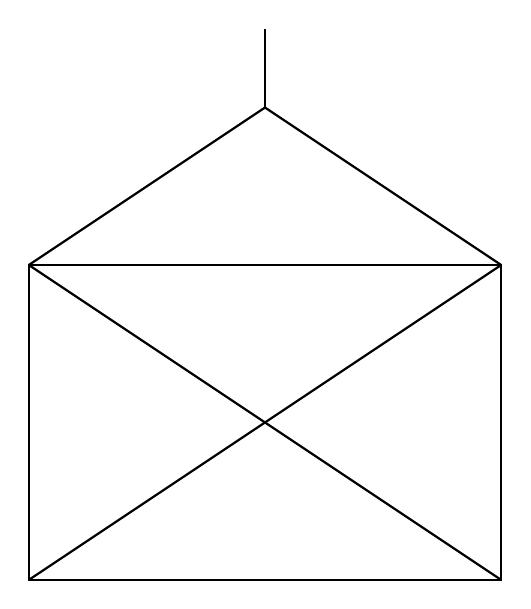
\begin{tikzpicture}
        \draw[thick] (0,0) rectangle (6,4);
        \draw[thick] (0,0) -- (6,4);
        \draw[thick] (0,4) -- (6,0);
        \draw[thick] (0,4) -- (3,6);
        \draw[thick] (6,4) -- (3,6);
        \draw[thick] (3,6) -- (3,7);
      \end{tikzpicture}
    }\hfil
    \resizebox{0.25\textwidth}{4cm}{
      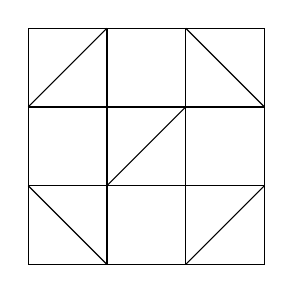
\begin{tikzpicture}
        \draw (0,0) rectangle (3,3);
        \draw (0,1) -- (3,1);
        \draw (0,2) -- (3,2);
        \draw (1,0) -- (1,3);
        \draw (2,0) -- (2,3);
        \draw (0,2) -- (1,3);
        \draw (2,3) -- (3,2);
        \draw (0,1) -- (1,0);
        \draw (2,0) -- (3,1);
        \draw (1,1) -- (2,2);
      \end{tikzpicture}
    }



  \itm{4.1.2} If possible, draw an eulerian graph \(G\) with \(v\) even and \(\varepsilon\) odd; otherwise, explain why there is no such graph.



  \itm{4.2.2} A mouse eats his way through a \(3 \times 3 \times 3\) cube of cheese by tunnelling through all of the 27 \(1 \times 1 \times 1\) subcubes.  If he starts at one corner and always moves on to an uneaten subcube, can he finish at the centre of the cube?



  \itm{4.2.3} Show that if \(G\) has a Hamilton path then, for every proper subset \(S\) of \(V\), \(\omega(G-S) \leq |S|+1\).

\end{itemize}
\end{document}
